\documentclass[10pt,conference,compsocconf]{IEEEtran}

\usepackage{hyperref}
\usepackage{graphicx}	% For figure environment
\usepackage{placeins}


\begin{document}
\title{Machine Learning Project I}

\author{
  Andres Montero, Elias Poroma, Jonas J\"aggi\\
  \textit{School of Computer and Communication Sciences, EPFL, Switzerland}
}

\maketitle

\begin{abstract}
  Machine learning is a field of artificial intelligence that uses statistical 
  techniques to give computer systems the ability to "learn" from data, 
  without being explicitly programmed. And in this project it is applied 
  to estimate the likelihood that a given data set is the result of a
  specific particle, for example the Higss Boson.
  This report gives an overview of six machine learning methods implemented
  to obtain the predictions and the results. It describes the pre-processing, 
  data cleaning and algorithms used in order to obtain a more significant 
  information.
  Comparing these results, the machine learning method that gives the 
  lowest error and therefore the best approximation is BEST METHOD !.

\end{abstract}

\section{Introduction}

The Higgs boson is an elementary particle in the Standard Model of 
particle physics, produced by the quantum excitation of the higgs field
and explains why some particles have mass~\cite{wiki01}. To confirm 
the existence of this particle, the CERN made several experiments from 
which we obtained real data and the objective of this work is to present 
a machine learning model that will give the best fit to the data provided.
However the data also contains other possible particles, so the main 
objective is to determine if the data of each experiment belongs to 
the higss boson or to other particle depending on the values provided
on the data set. For this purpose two data sets are provided, one to 
be used as the training data and the other as the testing data. 
The train data contains N=250000 measurements, where each of this
is described by 30 features and the output, which is 's' correct positive
or 'b' false positive. The test data contains 568.268 measurements with
the same 30 features and the output to be determined by the machine
learning model. The results of this work will be uploaded to kaggle ~\cite{kaggle01}, 
which will evaluate the results presented and provide a score of the 
model.

\section{Pre-Processing of Data}

\label{sec:Pre-Processing of Data}

Before apply any machine learning model it is really important that 
the data is understood and that the noise existing in the data is clean, 
this means that if there are incorrect or missing values, correlated or
categorical values, it is needed to filter/correct them otherwise
they may impact in a negative way in our prediction.

\subsection{Understanding the Data}
In the data presented there are 30 features, which are explained in 
the paper of the Higgs Challenge ~\cite{higgs_challenge01}. After a 
close analysis of this information, the results are:

\begin{itemize}
 \label{text:categorical}
\item The feature in column 22 \texttt{PRI\_jet\_num} is a categorical feature,
with discrete values of (0,1,2,3). For this reason it should be considered
for categorization and extracted from the data.
\item Depending on the values of \texttt{PRI\_jet\_num}  we have other columns
where the value is undefined, therefore this columns should be dropped 
on each categorical training.
\item Even after the removal of the undefined columns depending on the
categorical values we still find values that are undefined -999, which delivers
noise to the model, so they are replaced with the mean of the column is each
case.
\item After that we need to remove the outliers values, as we are using models
depending on MSE which penalizes heavily the outliers values, for this we use
the IQR technique ~\cite{IQR01}.

\end{itemize}

\subsection{Polynomials, Standardization, Offset}
 \label{text:datasteps}
\begin{itemize}
\item Polynomials are used in the models because linear models may cause
underfiting, however the degree of the polynomials should be calibrated carefully
to avoid over-fitting.
\item Once the polynomials are ready it is needed to standardize the data 
as the models we used converge faster with this feature, for this purpose 
the values (mean, standard deviation) from the train data  are used.
\item Adding one vector of "ones" as the offset in the data set also know as the
"bias" term.

\end{itemize}
\section{Models-Machine Learning}
For this project we implemented 6 different models to make the predictions, 
and for each one of them we implemented cross validation to assure that the 
model will work as expected with new values. For this we implemented k-fold 
cross validation with a values of k=5 to split the data in 5 even groups, where 
4 groups are used for training and one group is used for test. 
The results found for the different six models are summarized in Table~\ref{tab:models}.
As it can be understood from the table the best model is ``Best Model'', so this will
be the model used to describe in detail the process to achieve the result obtained.
To begin with the training of our model first we analyzed different scenarios: 

\begin{enumerate}
\item Training the model - Standardization \\
First the model trained with the entire set of data, without applying categorical 
training. In this case is only applied standardization as explained in ~\ref{text:datasteps}
The results obtained are:
1. RMSE:    2. Kaggle: 
With these results we clearly deduct that more cleaning stages were necessary to understand
the data and achieve that our model behaves as expected.

\item Training the model - Removing Outliers \\
Analyzing the previous step, we realized that the model showed really high values, to fix
this problem we proceed with the removing outliers step explained in ~\ref{text:datasteps}.
The results obtained are:
1. RMSE:    2. Kaggle: 
And it shows and improvement of \texttt{00\%}
\item Training the model - Categorical values \\
 Finally to obtain the official result presented to kaggle the model will trained depending
 on the categorical values as explained~\ref{text:categorical}
 The results obtained are:
 1. RMSE:    2. Kaggle:
 Which compared to the step 1 shows and improvement of \texttt{00\%}.
\end{enumerate}

\begin{table}[h]
  \caption{Models to Use.}
  \label{tab:models}
\begin{tabular}{|l|l|l|l|}
\hline
\textbf{Model}                                                              & \textbf{RMSE} & \textbf{Hyper Param}                                      & \textbf{gamma, iterations} \\ \hline
\begin{tabular}[c]{@{}l@{}}Least Squeares\\   GD\end{tabular}               & 8             & \begin{tabular}[c]{@{}l@{}}degree=\\ lambda=\end{tabular} & 1, 1          \\ \hline
\begin{tabular}[c]{@{}l@{}}Least Squeares\\   SGD\end{tabular}              & 8             & \begin{tabular}[c]{@{}l@{}}degree=\\ lambda=\end{tabular} & 1, 1         \\ \hline
Least Squeares                                                              & 8             & \begin{tabular}[c]{@{}l@{}}degree=\\ lambda=\end{tabular} & -          \\ \hline
\begin{tabular}[c]{@{}l@{}}Ridge\\   Regression\end{tabular}                & 8             & \begin{tabular}[c]{@{}l@{}}degree=\\ lambda=\end{tabular} & -          \\ \hline
\begin{tabular}[c]{@{}l@{}}Logistic\\   Regression\end{tabular}             & 8             & \begin{tabular}[c]{@{}l@{}}degree=\\ lambda=\end{tabular} & 1, 1          \\ \hline
\begin{tabular}[c]{@{}l@{}}Regularized\\   Logistic Regression\end{tabular} & 8             & \begin{tabular}[c]{@{}l@{}}degree=\\ lambda=\end{tabular} & 1, 1        \\ \hline
\end{tabular}
\end{table}


\section{BEST MODEL Detailed Description}
As we observed in the previous section the best model that fits 
the data is BEST MODEL, therefore a detailed explanation of the 
method and the code is explained:\\
To start the weights are initialized as a column of ones, then we define 
that all the data processing functions are true, as discussed before gives
a better result. Then we input the value for the selected model and define
the maximum iterations and start the cross validation step to assure that
the models will work as expected. Once this is completed a grid search
method is applied for the degree of the polynomials and also for the best
lambda used to penalize the model and avoid over-fitting in case that the 
degree found in the grid search is to high. The result shows that the best degree
is 2  and the best lambda is VALUE as you can see in the figure ~\ref{fig:best_degree}. 
With these results it is deduced that the lambda value is almost zero
which could cause that the model over-fits if the degree of the polynomial was
higher, however with just a value of two in the degree, the risk of over-fitting is
low, therefore the lambda value will be omitted. 
Once the best hyper-parameters are found the model can start with the training
for each of the categorical values, giving a prediction to each categorical value
and appending this to final result that will be saved as an excel file.



\begin{figure}[h]
  \centering
  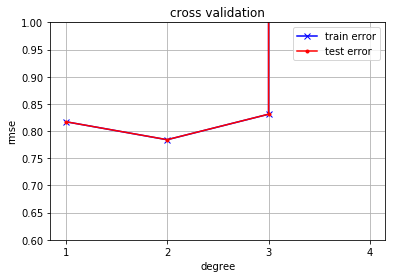
\includegraphics[width=\columnwidth]{cross_validation_degree}
  \caption{RMSE for different degrees of polynomial expansion - Ridge regression.}
  \vspace{-3mm}
  \label{fig:best_degree}
\end{figure}


\begin{figure}[h]
  \centering
  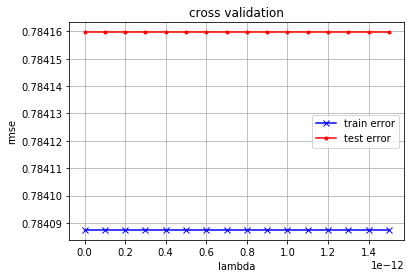
\includegraphics[width=\columnwidth]{cross_validation_lambda}
  \caption{RMSE for different regularization values - Ridge regression}
  \vspace{-3mm}
  \label{fig:best_lambda}
\end{figure}

\begin{table}[h]
  \caption{Significance of feature engineering}
  \label{tab:models}
\begin{tabular}{|l|l|l|l|}
\hline
\textbf{Data treatment}                                                              & \textbf{Training set division}                                      & \textbf{Kaggle score} \\ \hline
\begin{tabular}[c]{@{}l@{}}only standardization \& offset\end{tabular}                            & \begin{tabular}[c]{@{}l@{}}no division\end{tabular} & ???          \\ \hline
\begin{tabular}[c]{@{}l@{}}+ outlier replacement\end{tabular}                           & \begin{tabular}[c]{@{}l@{}}no division\end{tabular} & 0.65773          \\ \hline
+ outlier replacement                                                                           & \begin{tabular}[c]{@{}l@{}}division into \\jet categories\end{tabular} & ???          \\ \hline
\end{tabular}
\end{table}



  Scientific papers usually begin with the description of the problem,
justifying why the problem is interesting. Most importantly, it argues
that the problem is still unsolved, or that the current solutions are
unsatisfactory. This leads to the main gist of the paper, which is
``the idea''. The authors then show evidence, using derivations or
experiments, that the idea works. Since science does not occur in a
vacuum, a proper comparison to the current state of the art is often
part of the results. Following these ideas, papers usually have the
following structure:
\begin{description}
\item[Abstract] \ \\
  Short description of the whole paper, to help the
  reader decide whether to read it.
\item[Introduction] \ \\
  Describe your problem and state your
  contributions.
\item[Models and Methods] \ \\
  Describe your idea and how it was implemented to solve
  the problem. Survey the related work, giving credit where credit is
  due.
\item[Results] \ \\
  Show evidence to support your claims made in the
  introduction.
\item[Discussion] \ \\
  Discuss the strengths and weaknesses of your
  approach, based on the results. Point out the implications of your
  novel idea on the application concerned.
\item[Summary] \ \\
  Summarize your contributions in light of the new
  results.
\end{description}


\section{Tips for Good Writing}
\label{sec:tips-writing}

The ideas for good writing have come
from~\cite{editor10,jones08,anderson04}.

\subsection{Getting Help}
One should try to get a draft read by as many friendly people as
possible. And remember to treat your test readers with respect. If
they are unable to understand something in your paper, then it is
highly likely that your reviewers will not understand it
either. Therefore, do not be defensive about the criticisms you get,
but use it as an opportunity to improve the paper. Before your submit
your friends to the pain of reading your draft, please \emph{use a
  spell checker}.

\subsection{Abstract}
The abstract should really be written last, along with the title of
the paper. The four points that should be covered~\cite{jones08}:
\begin{enumerate}
\item State the problem.
\item Say why it is an interesting problem.
\item Say what your solution achieves.
\item Say what follows from your solution.
\end{enumerate}

\subsection{Figures and Tables}

\begin{figure}[tbp]
  \centering
  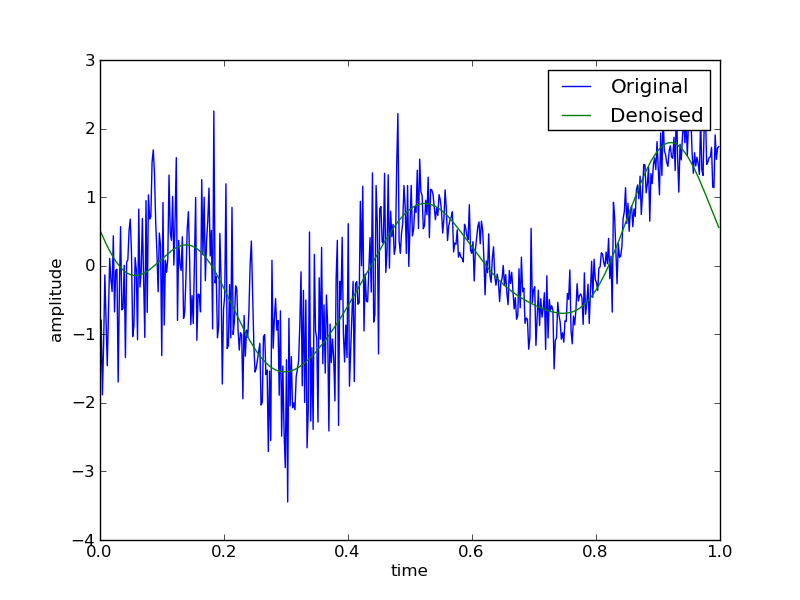
\includegraphics[width=\columnwidth]{denoised_signal_1d}
  \caption{Signal compression and denoising using the Fourier basis.}
  \vspace{-3mm}
  \label{fig:denoise-fourier}
\end{figure}
\begin{figure}[htbp]
  \centering
  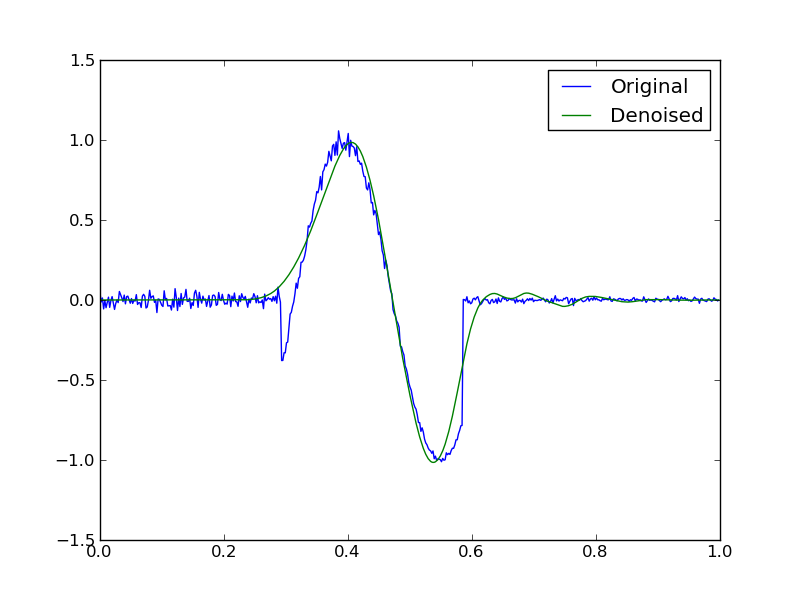
\includegraphics[width=\columnwidth]{local_wdenoised_1d}
  \vspace{-3mm}
  \caption{Signal compression and denoising using the Daubechies wavelet basis.}
  \label{fig:denoise-wavelet}
\end{figure}

Use examples and illustrations to clarify ideas and results. For
example, by comparing Figure~\ref{fig:denoise-fourier} and
Figure~\ref{fig:denoise-wavelet}, we can see the two different
situations where Fourier and wavelet basis perform well. 

\subsection{Models and Methods}
The models and methods
section should describe what was
done to answer the research question, describe how it was done,
justify the experimental design, and
explain how the results were analyzed.

The model refers to the underlying mathematical model or structure which 
you use to describe your problem, or that your solution is based on. 
The methods on the other hand, are the algorithms used to solve the problem. 
In some cases, the suggested method directly solves the problem, without having it 
stated in terms of an underlying model. Generally though it is a better practice to have 
the model figured out and stated clearly, rather than presenting a method without specifying 
the model. In this case, the method can be more easily evaluated in the task of fitting 
the given data to the underlying model.

The methods part of this section, is not a step-by-step, directive,
protocol as you might see in your lab manual, but detailed enough such
that an interested reader can reproduce your
work~\cite{anderson04,wavelab}.

The methods section of a research paper provides the information by
which a study's validity is judged.
Therefore, it requires a clear and precise description of how an
experiment was done, and the rationale
for why specific experimental procedures were chosen.
It is usually helpful to
structure the methods section by~\cite{kallet04methods}:
\begin{enumerate}
\item Layout the model you used to describe the problem or the solution.
\item Describing the algorithms used in the study, briefly including
  details such as hyperparameter values (e.g. thresholds), and
  preprocessing steps (e.g. normalizing the data to have mean value of
  zero).
\item Explaining how the materials were prepared, for example the
  images used and their resolution.
\item Describing the research protocol, for example which examples
  were used for estimating the parameters (training) and which were
  used for computing performance.
\item Explaining how measurements were made and what
  calculations were performed. Do not reproduce the full source code in
  the paper, but explain the key steps.
\end{enumerate}

\subsection{Results}

Organize the results section based on the sequence of table and
figures you include. Prepare the tables and figures as soon as all
the data are analyzed and arrange them in the sequence that best
presents your findings in a logical way. A good strategy is to note,
on a draft of each table or figure, the one or two key results you
want to address in the text portion of the results.
The information from the figures is
summarized in Table~\ref{tab:fourier-wavelet}.

\begin{table*}[htbp]
  \centering
  \begin{tabular}[c]{|l||l|l|l|}
    \hline
    Basis&Support&Suitable signals&Unsuitable signals\\
    \hline
    Fourier&global&sine like&localized\\
    wavelet&local&localized&sine like\\
    \hline
  \end{tabular}
  \caption{Characteristics of Fourier and wavelet basis.}
  \label{tab:fourier-wavelet}
\end{table*}

When reporting computational or measurement results, always
report the mean (average value) along with a measure of variability
(standard deviation(s) or standard error of the mean).


\section{Tips for Good Software}
\label{sec:tips-software}

There is a lot of literature (for example~\cite{hunt99pragmatic} and
\cite{spolsky04software}) on how to write software. It is not the
intention of this section to replace software engineering
courses. However, in the interests of reproducible
research~\cite{schwab00}, there are a few guidelines to make your
reader happy:
\begin{itemize}
\item Have a \texttt{README} file that (at least) describes what your
  software does, and which commands to run to obtain results. Also
  mention anything special that needs to be set up, such as
  toolboxes\footnote{For those who are
  particularly interested, other common structures can be found at
  \url{http://en.wikipedia.org/wiki/README} and
  \url{http://www.gnu.org/software/womb/gnits/}.}.
\item A list of authors and contributors can be included in a file
  called \texttt{AUTHORS}, acknowledging any help that you may have
  obtained. For small projects, this information is often also
  included in the \texttt{README}.
\item Use meaningful filenames, and not \texttt{temp1.py},
  \texttt{temp2.py}. 
\item Document your code. Each file should at least have a short
  description about its reason for existence. Non obvious steps in the
  code should be commented. Functions arguments and return values should be described.
\item Describe how the results presented in your paper can be reproduced.
\end{itemize}


\subsection{\LaTeX{} Primer}
\label{sec:latex-primer}

\LaTeX{} is one of the most commonly used document preparation systems
for scientific journals and conferences. It is based on the idea
that authors should be able to focus on the content of what they are
writing without being distracted by its visual presentation.
The source of this file can be used as a starting point for how to use
the different commands in \LaTeX{}. We are using an IEEE style for
this course.

\subsubsection{Installation}

There are various different packages available for processing \LaTeX{}
documents.
On OSX use Mac\TeX{}
(\url{http://www.tug.org/mactex/}). On Windows, use for example Mik\TeX{} (\url{http://miktex.org/}).

\subsubsection{Compiling \LaTeX{}}
Your directory should contain at least~4 files, in addition to image
files. Images should be in \texttt{.png}, \texttt{.jpg} or
\texttt{.pdf} format.
\begin{itemize}
\item IEEEtran.cls
\item IEEEtran.bst
\item groupXX-submission.tex
\item groupXX-literature.bib
\end{itemize}
Note that you should replace groupXX with your chosen group name.
Then, from the command line, type:
\begin{verbatim}
$ pdflatex groupXX-submission
$ bibtex groupXX-literature
$ pdflatex groupXX-submission
$ pdflatex groupXX-submission
\end{verbatim}
This should give you a PDF document \texttt{groupXX-submission.pdf}.

\subsubsection{Equations}

There are three types of equations available: inline equations, for
example $y=mx + c$, which appear in the text, unnumbered equations
$$y=mx + c,$$
which are presented on a line on its own, and numbered equations
\begin{equation}
  \label{eq:linear}
  y = mx + c
\end{equation}
which you can refer to at a later point (Equation~(\ref{eq:linear})).

\subsubsection{Tables and Figures}

Tables and figures are ``floating'' objects, which means that the text
can flow around it.
Note
that \texttt{figure*} and \texttt{table*} cause the corresponding
figure or table to span both columns.



\section{Summary}

The aim of a scientific paper is to convey the idea or discovery of
the researcher to the minds of the readers. The associated software
package provides the relevant details, which are often only briefly
explained in the paper, such that the research can be reproduced.
To write good papers, identify your key idea, make your contributions
explicit, and use examples and illustrations to describe the problems
and solutions.

\section*{Acknowledgements}
The author thanks Christian Sigg for his careful reading and helpful
suggestions.

\bibliographystyle{IEEEtran}
\bibliography{literature}

\end{document}
